\documentclass[11pt]{scrartcl}
\usepackage[parfill]{parskip}
\usepackage{graphicx}
\usepackage{booktabs}
\usepackage{tabulary}

\title{\textbf{Metrics for SCM Analysis}}
\subtitle{Project Evaluation}
\author{Ricardo García Fernández}
\date{\today}

\begin{document}

\maketitle

\tableofcontents

\newpage

\section{foobar: Big picture}

\emph{foobar}: Is a Software Development Company focussed in web data mining applications and result interpretation.

\par Delevop analysis from social media networks, crawlers and issue trackers to convert all the information to a human-readable solution for our clients. As some examples we are expertise in issue trackers visualization chars tools to convert the information into graphic that assist the project manager to make decisions faster and easily with just a look.

\section{Integrate VCS}

We need to implement a forge because our developers are in different physical locations and want to intergrate all development and managing tools for more efficient management.

The tools that we want to integrate are:

\begin{itemize}
    \item Version Control System VCS
    \item Issue Tracker
    \item Mail Server
    \item Continuous Integration Test
    \item Code Quality Analyzer
\end{itemize}

In this analysis we will begin the search for a VCS to suit our requirements.

\section{VCS}

\par \textbf{VCS}: Version Control System. Un Sistema de Control de Versiones es una herramienta para la gestión de los archivos y su ciclo de vida dentro de un proyecto. Gestiona todas las acciones que se realizan sobre ellos, crear, guardar, copiar, borrar, mover. La información queda reflejada en una base de datos, creando un histórico y ofreciendo una gestión ágil de los recursos a los usuarios.

\par Vamos a implantar un Control de Versiones para el trabajo en nuestra empresa de desarrollo de software mediante el análisis de unas métricas establecidas adaptadas a nuestros requerimientos.

\subsection{Subversion: SVN}

\textbf{Subversion}\footnote{http://subversion.tigris.org/}: is a FLOSS\footnote{Free Libre Open Source Software} Version Control System. It was created in 2000 by the company Collabnet belonging to the Apache Foundation.

\par SVN is the VCS most used in FLOSS\footnote{http://www.ohloh.net/repositories/compare} and private proyects as a Source Code Management (SCM) tool

\subsection{Git}

\subsection{CVS}

\section{Requirements}

Our initial requirements for the election of VCS tool are:

\begin{itemize}
    \item GUI Management Tools.
    \item Integration with IDEs.
    \item Mature and Stable versions.
    \item Lower learning curve.
    \item Success cases.
    \item License.
    \item Backup and restore.
    \item Migration guide.
    \item fork easily.
\end{itemize}

These requeriments has to become metrics because in this way we can evaluate with a technical and standard process.

\section{Metrics: Analysis}

Metrics: These are a set of measurable attributes that provide quantifiable information for the test result.

\par It is to define a set of metrics to evaluate the VCS projects and be able to quantify the final note. In this way, we obtain a numerical result of the project under review.

\par This result can be compared by analyzing other existing solutions to our problem.
Comparisons are made with the results obtained from the same premises for different version control systems and thus enables us to choose the most appropriate by value representation.

\subsection{OpenBRR Model}

\par Exist some analysis project models such OpenBRR which this analysis is based

\par OpenBRR was created as a project of unification of metrics for software projects. This model is considered free as it is project-oriented Free Software (FLOSS). Born in the year 2005 for this purpose but, as its website indicates, has failed to create a large community around.

\par Gives freedom when scoring each metric by a score of 1-5. Each section is divided to be more specific sub-metrics. Next, specific weight is given to each and thus be given greater weight to the metric that is considered more important by the user of the model. Generates output suitable for analysis.

\par The weight of the resulting metric provides personalized for the user and therefore nearest and manageable. For example: if the metric of documentation has a weight of 50 \% as opposed to security-related metrics with 10 \%, we are seeking a Software documentation which is the most important for our project and so both after data collection surely choose who has obtained the highest score with respect to documentation. It is an example roughly but quite clear. The weight is the most important because the final result depends on the value that we give to each section or metric. Thus we have an outcome directly related to our initial requirements.

\par We adapted OpenBRR model using scoring one to five (without 0 value) for each defined metric thus give us a wide range of possibilities and scalability to match a good result.

\subsection{Metrics chosen}

\par We have chosen a set of metrics to represent the most important values ​​related to file management. This set is specific for evaluating software so we can reuse most metrics obtained for other software projects.

\par Extending the model \emph{OpenBRR} have added some new metrics and eliminated other in order to create the specific model for our case.

\begin{tabular}{|l|}
    \hline {\bf Category}\\
    \hline Initial Analysis\\
    \hline Functionality\\
    \hline Usability\\
    \hline Robustness\\
    \hline Development\\
    \hline Community\\
    \hline Documentation\\
    \hline
\end{tabular}

\subsection{Weight \& Punctuation}

After analyzing the requirements and scoring metrics, we proceed to give a weight to each section defined in the document. The weight given is what gives the final value that the user seeks to create a subjective result from an objective score. That is, to adapt to the needs of the company to the product being analyzed.

We defined the weight given to each category in the table below:

\begin{tabular}{|l|l|}
    \hline Category & Weight\\
    \hline Initial Analysis	 & 13,00\%\\
    \hline Functionality & 12,00\%\\
    \hline Usability & 14,00\%\\
    \hline Robustness & 17,00\%\\
    \hline Development & 15,00\%\\
    \hline Community & 19,00\%\\
    \hline Documentation & 10,00\%\\
    \hline
\end{tabular}

\par You can see that the value that is given more weight is Community with 19 \%, followed Robustness with 17 \% and Development with 15 \%. 

\subsubsection{Community, Robustness and Development}

\par We can see how the metric highlights related \emph{Community} because being a FLOSS project depend in part on the interaction of the community, ie the health of it. At first it seems to be in good health because of its history but in recent years has been decreasing the work reflected in the community regarding email lists and commits per month. It can also be noted that the initial development team is not present in the current development of an active but this has not affected the development. There has been renewed core providing strength to the project developers.

\begin{figure}
  \centering
    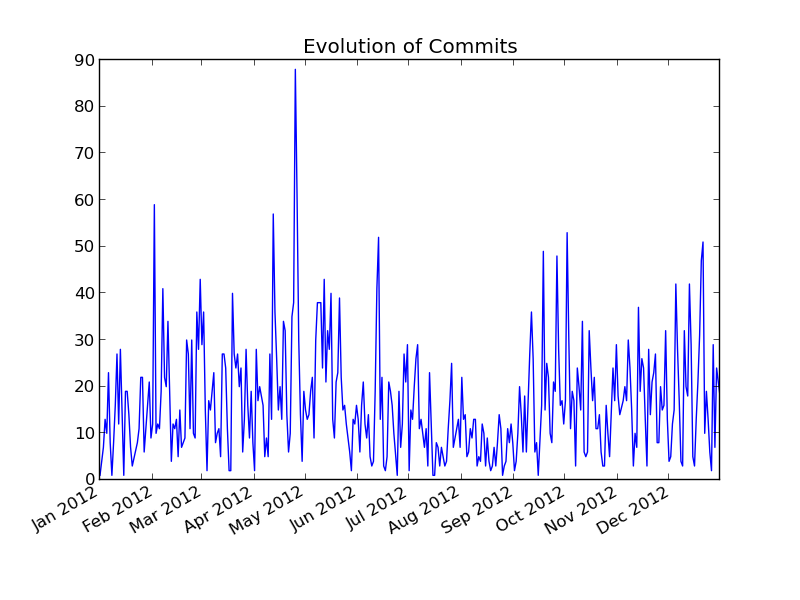
\includegraphics[width=0.8\textwidth]{libcsvanaly2/script_sample/basic_timeseries.png}
  \caption{Commit evolution during 2012}
  \label{fig:2012-monthy-commmits}
\end{figure}

\begin{itemize}
    \item Avg commits per month, last six months.
        \begin{itemize}
            \item Compare with other projects or \textbf{itself with other year results}. Comparision with six month and twelve earlier.
            \item \textbf{Result}: Less work than a year before on total commits (-,-,-,-,-,+) as show in figure~\ref{fig:2012-monthy-commmits}:
        \end{itemize}
    \item Avg monthly volumen of general mailing lists during the last six months
    \begin{itemize}
        \item Compare with other projects or itself with other year results. Table from 2012:

            \begin{tabular}{|l|l|l|l|l|l|}
                \hline
        	    Jan (4.5M) & Feb (2.5M) & Mar (3.5M) & Apr (2.1M) & May (1.8M) & Jun (1.8M)\\
        	    \hline
        	    - & + & - & - & - & -\\
                \hline
                Jul (1.4M) & Aug (3.3M) & Sep (1.9M) & Oct (1.7M) & Nov (1.7M) & Dec (497K)\\
                \hline
            \end{tabular}
        \item \textbf{Decreases}.
    \end{itemize}
    \item Developers that left the project and those that started to participate (last year) (and also for the core team)
    \begin{itemize}
        \item Started to participate las year: \textbf{6}
    \end{itemize}
	    \item Knowledge concentration (territoriality): In 2012 year we can assume a territoriality over 80\% with 8538 actions from the total of 10417 in files per one developer, so 81,96\%.
    \item Is still the original developer/team active nowadays? Yes, innactive.
    \begin{itemize}
        \item How did affect the project ? commits avg continued normal ?
        \item Yes, the core team continues in the project but not with the same weight. This not affects the repository because committs per month is constant.
    \end{itemize}
\end{itemize}

\par By the \emph{Robustness} can say that this is a complete project. We say this after observing the care that is in each of the versions that have been published and the treatment given to them. It keeps alive a previous version (1.6) only if there are security errors while development continues forward with the current version (1.7) fixing bugs and releasing each patch with an average of two months. These data were collected for 2012.

\begin{itemize}
    \item Versions

        \begin{tabular}{|l|l|l|l|}
            \hline
                {\bf Version} & {\bf Date} & {\bf History} & {\bf Problems solved}\\
            \hline
                1.7.x & October 11, 2011 & Fully supported & Fixes for all bugs\\
            \hline
                1.6.x & March 20, 2009 & Partially supported & Only fixes for security issues and bugs which could cause data loss\\
            \hline
                1.5.x & June 19, 2008 and earlier & No longer supported & No longer supported\\
            \hline
        \end{tabular}

    \item Num. point/patch releases last year
    \begin{itemize}
        \item Number of releases is constant ? depends of the year ? Public roadmap for next versions\footnote{http://subversion.apache.org/roadmap.html}.
        \item Patches in last year is constant ? Average: two months\footnote{http://subversion.apache.org/docs/release-notes/release-history.html}.

            \begin{tabular}{|l|l|l|}
                \hline Version & Date & Information\\
                \hline 1.7.8 & (Thursday, 20 December 2012) & Bugfix release.\\
                \hline 1.7.7 & (Tuesday, 9 October 2012) & Bugfix release.\\
                \hline 1.7.6 & (Wednesday, 15 August 2012) & Bugfix release.\\
                \hline 1.7.5 & (Thursday, 17 May 2012) & Bugfix/security release.\\
                \hline 1.7.4 & (Thursday, 8 March 2012) & Bugfix release.\\
                \hline 1.7.3 & (Monday, 13 February 2012) & Bugfix release.\\
                \hline
            \end{tabular}
    \end{itemize}
\end{itemize}

\par Regarding \emph{Development} we see that the score is good because it has various APIs (in various programming languages ​​C and Java are the most widespread\footnote{http://www.ohloh.net/languages/compare?measure=loc\_changed\&percent=true} and demanded in the market\footnote{http://www.tiobe.com/index.php/content/paperinfo/tpci/index.html}) and is used in external projects so it is a widespread practice. But of course, you have to know how to program in order to understand the API.

\begin{itemize}
    \item Project API in the same web - Client for Java and C.
    \item Easy understanding - Easy understanding for Software Developers. 
    \item Is it used in other projects not directly related? - Yes, from extra plugins, functionalities, integrated in aplications and forges.
\end{itemize}
  
\par The documentation included in the development is extensive and clear. There are various examples to initialize repositories and projects. The manuals include examples related to each option and the documentation is clear and concise. Svnbook has a book in different languages. Reading the book helps a lot in making contact with the tool. By the offline help, not much beyond the command \textbf{man} (own documentation of a tool), where there are no good examples of use.

\begin{itemize}
    \item Online tutorials - Development\footnote{http://subversion.apache.org/docs/} and API documentation too.
    \item Offline tutorials - SVNBook\footnote{http://svnbook.red-bean.com/}
    \item Hello World - Tutorial to initialize a Repository in 10 minutes.
    \item Books from the author, authors or company -  SVNBook
    \item Languages - Various Languages (Deutsch | English | French | Spanish | Italian | Japanese | Norwegian | Portuguese | Russian | Chinese)
\end{itemize}

\par En un segundo grupo podemos ver que aparecen Usability 14\%, Initial Analysis 13\% y Functionality 12\%.

\subsubsection{Usability, Initial Analysis and Functionality}

\par \emph{Usability}, in this case we refer to the usability related to the interaction between the user and the tool. The server configuration is a highlight that we see in the inner section \emph{Client UI}. Several options are valid for the control management tool. Moreover we also observe that this tool is widespread and has a high learning curve but that you have to be a technical person to quickly take advantage of the functionality that presents Subversion.

\begin{itemize}
    \item UI client
	    \begin{itemize}
            \item Internal (server management) - Using \emph{svnadmin} command in server mode.
            \item Included - It's included in the installation.
            \item Extra plugin - Has extra plugin to apply this functionalities but not depends on it.
            \item Web client - User-Friendly SVN\footnote{http://www.usvn.info/} promoted by Collabnet.
        \end{itemize}

    \item Easy learning
	    \begin{itemize}
            \item Too technical - Not too much technical to use.
            \item Early adoption - Is the most VCS used around the world of Software Development.
            \item Low learning curve - Yes, it's easy to get in touch and work.
        \end{itemize}
\end{itemize}

\par \emph{Initial Analysis} section includes two important values​​, the license under which the software is released and the time it takes to launch the first repository. As part of the license is the Apache License v2.0\footnote{http://www.apache.org/licenses/LICENSE-2.0}. FLOSS License is an \emph{standard} that is compatible with \emph{GPLv3}\footnote{http://www.apache.org/licenses/GPL-compatibility.html}. The Apache License v2.0 gives us full control over the code and provide inputs to the official distribution by third parties.

\begin{itemize} 
    \item Private - \textbf{No}
    \item Free Software: Non standard (My own license) \textbf{No}
    \item Free Software: \textbf{Standard}. Included in list of most used FLOSS Licences in OSI\footnote{http://opensource.org/licenses/index.html} and FSF directory\footnote{http://www.gnu.org/licenses/license-list.en.html}.
    \item Dual Licensing: \textbf{No}
    \item Compatible with others - \textbf{Yes}: The result is a license that is supposed to be compatible with other open source licenses, while remaining true to the original goals of the Apache Group and supportive of collaborative development across both nonprofit and commercial organizations. The Apache Software Foundation is still trying to determine if this version of the Apache License is compatible with the GPL.\footnote{http://www.apache.org/licenses/GPL-compatibility.html}
\end{itemize}

\par The time of the first test is very critical as far as I'm concerned. We see that in a time frame of 10 to 30 minutes you publish a Subversion repository for user access. This time is a success as the first contact is the most important and time is not wasted. Publish a functional online repository in between 10 to 30 minutes.

\begin{itemize}
    \item \textgreater
4 hours
    \item 1-4 
    \item 30 min - 1 hour
    \item \textbf{10 - 30} - Install and publish the repository with \textbf{Apache} or \textbf{svnserve}\footnote{http://svnbook.red-bean.com/en/1.7/svn.ref.svnserve.html}.
    \item \textless
10 minutes
\end{itemize}

\par In the category \emph{Funcionality}, UI foremost ranks with 40 \% of the score. The multiple options to access Subversion repository management regardless of having the user level, make this tool your fast and easy access to the different types of users to be found.

\begin{itemize}
    \item Console client - Yes included.
    \item OS file explorer integration - Collabnet Tortoise SVN - http://tortoisesvn.tigris.org/ GPL)
    \item Graphic client - Tortoise SVN.
    \item Specific plugin for tools - Eclipse Plugin by Tigris: Subclipse - http://subclipse.tigris.org/
    \item Solution from the same company - Yes, Collabnet - http://www.usvn.info/ using Cecill License (GPL Compatible)
\end{itemize}

\par One point to note is related to \emph{Backup and restore}. This aspect has been very careful in Subversion. Includes a proprietary tool to manage copies of the database repository and a speedy recovery. Integrates with all operating systems and can be configured easily.

\begin{itemize}
    \item Nothing - \emph{Not necessary}.
    \item Workaround solution - \emph{Not necessary}.
    \item Extra plugin - \emph{Not necessary}.
    \item Included - \textbf{Yes}, has a tool to backup repository database included.
    \item Easily Configurable - \emph{Backup from svn database} using \emph{svnadmin dump} command total or incremental. Use \emph{svnadmin load} to restore backup version.
\end{itemize}

\par En el apartado de seguridad conocido como Profile management, vemos que la estructura de Subversion se divide en directorios, todo son directorios. Por lo que los permisos también se otorgan a partir de directorios, grupos y usuarios. Es el clásico sistema de permisos en el que nos ofrece una herramienta visual online USVN para que los no tan técnicos se despreocupen de configuraciones en el servidor y gestionen los grupos, usuarios y permisos sobre proyectos.

\par Finally the Documentation section with a weight of 10 \%. This section is also included within Development is valued so much documentation related to the development of the tool documentation as such.

\subsubsection{Documentation}

\par This section has weighed less in the total analysis. Notably, as we have done previously that has a very good online documentation for the services offered by the tool Subversion but takes more documentation offline.

\begin{itemize}
    \item Online tutorials - Development
    \item Offline tutorials - SVNBook
    \item Hello World - Init a Repository in 10 minutes
    \item Books from the author, authors or company - SVNBook
    \item Languages - Various Languages (Deutsch | English | French | Spanish | Italian | Japanese | Norwegian | Portuguese | Russian | Chinese)
\end{itemize}

\section{Results}

We can see that the result is a score of \textbf{4.29 out of 5}. This result is transferred to a score of \textbf{85.87 out of 100} (applying rounding to two decimal places for each calculation).

\begin{tabular}{|l|l|l|l|}
    \hline {\bf Category} & {\bf Weight} & {\bf Unweighted Rating} & {\bf Weighted Rating}\\
    \hline {\bf Initial Analysis}	 & 13,00\% & 4,06 & 0,53 \\
    \hline {\bf Functionality} & 12,00\% & 4,37 & 0,52\\
    \hline {\bf Usability} & 14,00\% & 4,67 & 0,65\\
    \hline {\bf Robustness} & 17,00\% & 4,61 & 0,78\\
    \hline {\bf Development} & 15,00\% & 4,47 & 0,67\\
    \hline {\bf Community} & 19,00\% & 3,65 & 0,69\\
    \hline {\bf Documentation} & 10,00\% & 4,4 & 0,44\\
    \hline
\end{tabular}

\par Following the model proposed by OpenBRR, the score of 100 is considered acceptable since it is within the range of 80 to 90 points. This score alone does not tell us much more than the number.

\par Now we have to make the comparison with other Version Control Systems using the same metrics described in the document. In this way we can obtain comparable numbers and choose the VCS that more suits our needs.

\section{Compare Results}

In the table below we can see a comparison of the results obtained from the analysis of the three possible solutions, \emph{SVN}, \emph{Git} and \emph{CVS} using \emph{Unweighted Rating (UR)} and \emph{Weighted Rating (WR)}:

\begin{tabular}{|l|l|l|l|l|l|l|l|}
    \hline
     &  & {\bf Subversion} &   & {\bf Git} &  & {\bf CVS} &  \\
    \hline
    {\bf Category} & {\bf Weight} & {\bf UR} & {\bf WR} & {\bf UR} & {\bf WR} & {\bf UR} & {\bf WR}\\
    \hline
    {\bf Initial Analysis} & 13,00\% & 4,06 & {\bf 0,53} & 3,12 & 0,41 & 4,06 & {\bf 0,53}\\
    \hline
    {\bf Functionality} & 12,00\% & 4,37 & 0,52 & 4,7 & {\bf 0,56} & 3,81 & 0,46\\
    \hline
    {\bf Usability} & 14,00\% & 4,67 & {\bf 0,65} & 3,53 & 0,49 & 3,93 & 0,55\\
    \hline
    {\bf Robustness} & 17,00\% & 4,61 & 0,78 & 4,73 & {\bf 0,8} & 3,03 & 0,52\\
    \hline
    {\bf Development} & 15,00\% & 4,47 & 0,67 & 4,67 & {\bf 0,7} & 3,78 & 0,57\\
    \hline
    {\bf Community} & 19,00\% & 3,65 & 0,69 & 4,1 & {\bf 0,78} & 1,96 & 0,37\\
    \hline
    {\bf Documentation} & 10,00\% & 4,4 & 0,44 & 5 & {\bf 0,5} & 3,3 & 0,33\\
    \hline
    {\bf Totals} & 100,00\% & 4,29 & {\bf 85,87} & 4,25 & 84,95 & 3,32 & 66,4\\
    \hline
\end{tabular}

\par At first glance it is seen that in the overall score \textbf{85.87 points} against \textbf{SVN} with minimal difference \textbf{Git 84.95}. CVS is relegated to a distant third with respect to both with 66.4 points.
At first glance it is seen that in the overall score \textbf{stands SVN}. \emph{SVN} gets a score of \textbf{85.87 points} with a minimum difference with \emph{Git}. \emph{Git} gets a score of \textbf{84.95 points}. \emph{CVS} is relegated to a distant third with respect to both with \textbf{66.4 points}.

\par For further analysis, we divided the analysis in the same groups previously selected by the representation of requirements through the weights.

\par Although at first glance it seems that will fight to the death between SVN and Git.

\subsubsection{Community, Robustness and Development}

\par Starting with the requirement for value, the \emph{Community}, we see that in Git community is healthier than SVN and CVS course. CVS community is clearly outweighed by SVN and Git for double score.

\par In \emph{Robustness} metric results we ​​can appreciate \emph{evenly between SVN and Git (0.78 vs. 0.8)}, whereas the score \emph{CVS sinks back to 0.52}. SVN and CVS are on par with this paragraph.

\par Finally, the results obtained by the metric associated with the development, you see, again, a near tie between \textbf{SVN and Git} with \emph{0.67 and 0.7 points respectively}. CVS \emph{falls again} relegated to last place with \textbf{0.57 points}, not as far back as in the above metrics. This metric is important because it includes the score related documentation and API. These two points have to be taken into account because \emph{we will have to work with them to integrate the VCS}.

\par We see that \textbf{Git} highlighted in this comprehensive set of metrics. Being the most important in relation to the initial requirements of the company.

\subsubsection{Usability, Initial Analysis and Functionality}

\par In this group of metrics, \emph{Usability} is the most valuated by its weight. In this case we see how \textbf{SVN with 0.65 points} clearly leads the standings ahead of \textbf{CVS} and \textbf{Git} with \emph{0.55 and 0.49 points} respectively. Usability in SVN very careful as we see in the results. Furthermore compared to other tools strengthens.

\par \emph{Initial Analysis} also led \textbf{SVN with 0.53 points tying with CVS}. One can say that being the oldest VCS weight we have given to the metrics relating to the qualities of the licenses they use and \emph{easy setup of applications} are best suited to the detriment of \textbf{Git with 0.41 points}. Maybe that's immaturity in Git.

\par By the \emph{Functionality} related metric can observe the good quality in \textbf{Git with 0.56 points}, \emph{followed by SVN and CVS} with \textbf{0.52 points with 0.46 points}. The quality of the functionality in Git can claim to be high, because it has exceeded two VCS score established for over ten years.

\par In this metrics group we can see that \textbf{SVN is above Git and CVS} regarding \emph{Usability, Funciolidad and Initial Analysis}. These qualities are important as \emph{they are the key for user interaction with the VCS tool} so we have to take into account these results to the overall analysis.

\subsubsection{Documentation}

\par The last group contains only the metric only documentation. Has been relegated to the last place because it has more value to that included in Development. It is important because it contains the manuals and the \emph{results of use and learning}.

\par Analyzing the results remains the general trend, \textbf{Git is in the lead with 0.5 points} while \textbf{SVN and CVS obtained 0.44 and 0.33 points respectively}. \emph{Documentation and help} in Git stands for the quantity and quality, as we might say in \emph{SVN}. The exception appears to \textbf{CVS}, it is not understandable that there is not level with the other two tools, being the oldest of the three, \emph{seems not to have been able to manage the knowledge of the tool}.

\section{Conclusions}

\section{Further work}

Resumen, que posibilidades se han dejado fuera y futuribles.
% TODO: maillist, bugtracker, standards, foundation, uses, succed, mentoring programs\footnote{http://subversion.apache.org/docs/community-guide/}.

\section{Analysis Document}

Analysis Document with all punctuations and comparisons between the three VCS could be found in github for dowloading:
\begin{itemize}
    \item https://github.com/ricardogarfe/mswl-project-evaluation/blob/master/final\_report/scm-metrics.sxc
\end{itemize}

Here is the full metric list and its punctuation explanation. If you are interested in changing the weights of the metrics, open the sxc scm-metrics file and access Book Category Ranking. There is a summary of the results so you can do a quick scan to your preference among the three VCS elected.

\par You can change the assigned weights according to their requirements, while the total is 100 course, traps are not enabled yet.

\par Feel free to add it believes appropriate VCS has been left out of the analysis. As can be the case of mercurial, Bazaar, etc. This way you can get a more complete and robust document so it can be reused by more people.

\section{Toolset}

\par Herramienta: es un instrumento que se utiliza para llevar a cabo un trabajo. En este caso la recolección de datos y el análisis son el trabajo realizado.

\par Para este análisis se han utilizado varias herramientas para conseguir la información necesaria.

\subsection{Data sources}

Data Sources from internet:

\begin{itemize}
    \item Website - http://subversion.apache.org/ \& http://subversion.tigris.org/
    \item Source code management system - svn co http://svn.apache.org/repos/asf/subversion subversion
    \item Releases - http://subversion.apache.org/packages.html
    \item Wikis - http://wiki.apache.org/subversion/
    \item Documentation - http://subversion.apache.org/docs/
    \item Mailing lists -http://subversion.apache.org/mailing-lists.html
    \item Bug tracking system - http://subversion.tigris.org/issue-tracker.html
    \item Irc channel - IRC on channel \#svn on irc.freenode.net
\end{itemize}

\subsection{Data mining Applications}

We used a pair of tools for obtaining related data repositories.

\par These two tools related to data mining are developed in python. Its main function is to make public information from a repository to a functional database with which you can easily obtain results about the activity of the community that the project develops.

\begin{itemize}
    \item CVSAnaly\footnote{https://github.com/MetricsGrimoire/CVSAnalY} - Herramienta para obtener información de un repositorio de código. Crea una base de datos con toda la información referente al repositorio, usuarios, commits, ficheros.
    \item libcvsanaly2\footnote{http://git.libresoft.es/libcvsanaly2} - Librería para generar informes a partir de la base de datos creada por CVSAnaly2 con respecto a las acciones sobre los ficheros de un repositorio.
\end{itemize}

\subsection{Repository of Repositories: RoR}

RoR are analysis repository tools. Display information about project communities: Committers, Groups, Application, Organizations, timelines in an easily visualization and configuration charts. For this analysis we used Ohloh.

\begin{itemize}
    \item Ohloh\footnote{http://www.ohloh.net/} - Is a RoR where there are 581,685 open source projects analyzed.
\end{itemize}

\section{Metrics: Full List}

\begin{enumerate}
    \item Initial Analysis
    \begin{itemize}
        \item License (Apache License, Version 2.0)
        \begin{itemize} 
            \item Private - \textbf{No}
            \item Free Software: Non standard (My own license)
            \item Free Software: \textbf{Standard} (included in list of most used FLOSS Licences)
            \item Dual Licensing: \textbf{No}
            \item Compatible with others - \textbf{Yes}: The result is a license that is supposed to be compatible with other open source licenses, while remaining true to the original goals of the Apache Group and supportive of collaborative development across both nonprofit and commercial organizations. The Apache Software Foundation is still trying to determine if this version of the Apache License is compatible with the GPL.\footnote{http://www.apache.org/licenses/GPL-compatibility.html}    
        \end{itemize}
	    \item Time for setup and installing to create a public/private repository II
        \begin{itemize}
            \item \textgreater
 4 hours
            \item 1-4 
            \item 30 min - 1 hour
            \item \textbf{10 - 30} - Install and publish the repository with \textbf{Apache} or \textbf{svnserve}\footnote{http://svnbook.red-bean.com/en/1.7/svn.ref.svnserve.html}.
            \item \textless
 10 minutes
        \end{itemize}
    \end{itemize}

    \item Functionality
        \begin{itemize}
	    \item UI client
            \begin{itemize}
                \item Console client - Yes included.
                \item OS file explorer integration - Collabnet Tortoise SVN - http://tortoisesvn.tigris.org/ GPL)
                \item Graphic client - Tortoise SVN.
                \item Specific plugin for tools - Eclipse Plugin by Tigris: Subclipse - http://subclipse.tigris.org/
                \item Solution from the same company - Collabnet - http://www.usvn.info/ Cecill License (GPL Compatible)
            \end{itemize}
	    \item Backup and restore (restore costs estimation or revert actions)
            \begin{itemize}
                \item Nothing - Not necessary.
                \item Workaround solution - Not necessary.
                \item Extra plugin - Not necessary
                \item Included - Yes, has a tool to backup repository database included.
                \item Easily Configurable - Backup from svn database using 'svnadmin dump' command total or incremental. Use 'svnadmin load' to restore backup version.
            \end{itemize}

	    \item Profile management 
            \begin{itemize}
                \item Workaround solution - Not necessary.
                \item Integrated profile management - Users in subversion had access to every repository.
                \item Directories - Profiles related to directory/user/groups access defined.
                \item Groups/users/directories - Profiles related to directory/user/groups access defined.
                \item Graphic Inteface tool - Tortoise, USVN, Eclipse Pluging.
            \end{itemize}
        \end{itemize}

    \item Usability
        \begin{itemize}
	    \item UI client
        	\begin{itemize}
                \item Internal (server management) - Using svnadmin command.
                \item Included - It's included in the installation.
                \item Extra plugin - Has extra plugin to apply this functionalities but not depends on it.
                \item Web client - User-Friendly SVN\footnote{http://www.usvn.info/} promoted by Collabnet.
            \end{itemize}

	    \item Easy learning
        	\begin{itemize}
                \item Too technical 
                \item Early adoption - Is the most VCS used around the world of Software Development.
                \item Low learning curve - Yes, it's easy to get in touch and work.
            \end{itemize}
        \end{itemize}

    \item Robustness

        \begin{itemize}
	    \item Mature and stable version - Yes.
	        \begin{itemize}
            \item Versions

                \begin{tabular}{|l|l|l|l|}
                    \hline
	                    {\bf Version} & {\bf Date} & {\bf History} & {\bf Problems solved}\\
                    \hline
	                    1.7.x & October 11, 2011 & Fully supported & Fixes for all bugs\\
                    \hline
	                    1.6.x & March 20, 2009 & Partially supported & Only fixes for security issues and bugs which could cause data loss\\
                    \hline
	                    1.5.x & June 19, 2008 and earlier & No longer supported & No longer supported\\
                    \hline
                \end{tabular}

            \end{itemize}

	    \item Num. point/patch releases last year
	        \begin{itemize}
                \item Number of releases is constant ? depends of the year ? Public roadmap for next versions\footnote{http://subversion.apache.org/roadmap.html}.
                \item Patches in last year is constant ? Average: two months\footnote{http://subversion.apache.org/docs/release-notes/release-history.html}.

                    \begin{tabular}{|l|l|l|}
                        \hline Version & Date & Information\\
                        \hline 1.7.8 & (Thursday, 20 December 2012) & Bugfix release.\\
                        \hline 1.7.7 & (Tuesday, 9 October 2012) & Bugfix release.\\
                        \hline 1.7.6 & (Wednesday, 15 August 2012) & Bugfix release.\\
                        \hline 1.7.5 & (Thursday, 17 May 2012) & Bugfix/security release.\\
                        \hline 1.7.4 & (Thursday, 8 March 2012) & Bugfix release.\\
                        \hline 1.7.3 & (Monday, 13 February 2012) & Bugfix release.\\
                        \hline
                    \end{tabular}
            \end{itemize}
        \end{itemize}

    \item Development 
    \begin{itemize}
	    \item API
    	    \begin{itemize}
                \item Project API in the same web - Client for Java and C.
                \item Easy understanding - Easy understanding for Software Developers. 
                \item Is it used in other projects not directly related? - Yes, from extra plugins, functionalities, integrated in aplications and forges.
            \end{itemize}

	    \item Documentation
    	    \begin{itemize}
                \item Online tutorials - Development
                \item Offline tutorials - SVNBook\footnote{http://svnbook.red-bean.com/}
                \item Hello World - Tutorial to initialize a Repository in 10 minutes.
                \item Books from the author, authors or company -  SVNBook
                \item Languages - Various Languages (Deutsch | English | French | Spanish | Italian | Japanese | Norwegian | Portuguese | Russian | Chinese)
            \end{itemize}
    \end{itemize}

    \item Community
    \begin{itemize}
	    \item Avg commits per month, last six months.
	        \begin{itemize}
                \item Compare with other projects or \textbf{itself with other year results}. Comparision with six month and twelve earlier.
                \item \textbf{Result}: Less work than a year before on total commits (-,-,-,-,-,+)
            \end{itemize}
	    \item Avg monthly volumen of general mailing lists during the last six months
	    \begin{itemize}
            \item Compare with other projects or itself with other year results. Table from 2012:

                \begin{tabular}{|l|l|l|l|l|l|}
                    \hline
            	    Jan (4.5M) & Feb (2.5M) & Mar (3.5M) & Apr (2.1M) & May (1.8M) & Jun (1.8M)\\
            	    \hline
            	    - & + & - & - & - & -\\
                    \hline
                    Jul (1.4M) & Aug (3.3M) & Sep (1.9M) & Oct (1.7M) & Nov (1.7M) & Dec (497K)\\
                    \hline
                \end{tabular}
            \item Decreases (-,+,-,-,-,-).
        \end{itemize}
	    \item Developers that left the project and those that started to participate (last year) (and also for the core team)
	    \begin{itemize}
            \item Started to participate las year: \textbf{6}
        \end{itemize}
	    \item Knowledge concentration (territoriality): In 2012 year we can assume a territoriality over 80\% with 8538 actions from the total of 10417 in files per one developer, so 81,96\%.
	    \item Is still the original developer/team active nowadays? Yes, innactive.
	    \begin{itemize}
            \item How did affect the project ? commits avg continued normal ?
            \item Yes, the core team continues in the project but not with the same weight. This not affects the repository because committs per month is constant.
        \end{itemize}
    \end{itemize}

    \item Documentation
    \begin{itemize}
 	    \item Several levels of documentation (user, development, translator, languages) III
     	    \begin{itemize}
                \item Online tutorials - Development
                \item Offline tutorials - SVNBook
                \item Hello World - Init a Repository in 10 minutes
                \item Books from the author, authors or company - SVNBook
                \item Languages - Various Languages (Deutsch | English | French | Spanish | Italian | Japanese | Norwegian | Portuguese | Russian | Chinese)
            \end{itemize}
    \end{itemize}

\end{enumerate}

\begin{thebibliography}{9}

\bibitem{subversion-site}
  Subversion Tigris,\\
  http://subversion.tigris.org/

\bibitem{subversion-apache}
  Subversion Apache,\\
  http://subversion.apache.org/

\end{thebibliography}

\end{document}
